%!TEX root =  ../main.tex

\chapterimage{Floating_Houses_Of_Malaysia} 
\mychapter{Circles}{circle}

Right triangles can be understood to a degree that is truly breath-taking.  With an
astoundingly low amount of information, the complete scenario can be flushed out.
This deep level of understanding is perhaps only known to cartographers and 
video game designers, but angles and distances could enrich all our lives.

How can you know if I tree will fall on your house?  Armed with only how far away
it is, and the angle from your eye to the top (and your eye's height) you can tell
how high the tree is.

\newpage
\chapterminitoc

%									9 - 1
\newpage
\section{Angles}
\noindent\makebox[\textwidth]{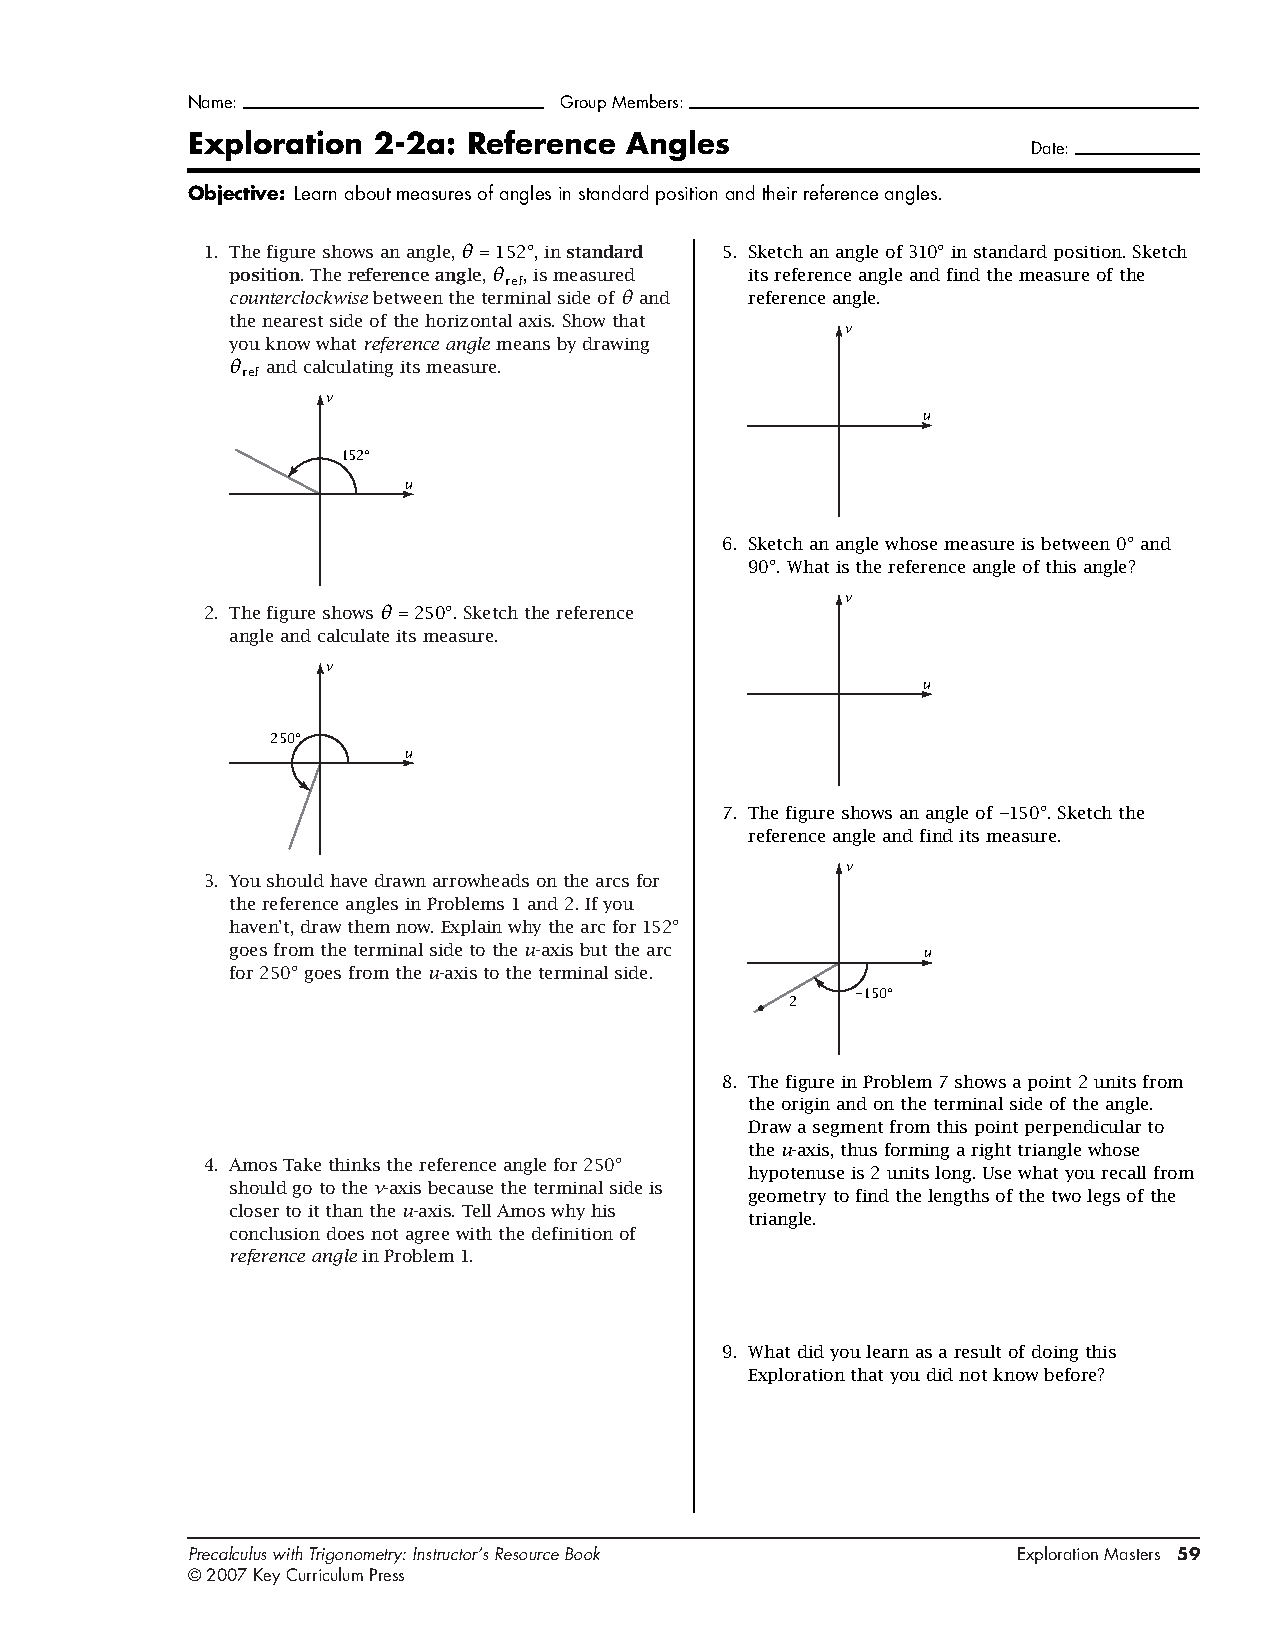
\includegraphics[width=\paperwidth]{ch09/0901p.pdf}}
%!TEX root =  ../main.tex

\subsection{Initial and Terminal}

\objective{Simplify angles and their coterminal synonyms, and apply them to the three basic trigonometric functions}


Angles are a measure of turning.  Since Babylonian times, it has been customary to divide
the circle into 360 parts, beginning directly off to the right, and proceeding counter-clockwise.
The beginning ray pointing right is known as the \textbf{initial side}, whereas the ray pointing
off where the angle has turned to is called the \textbf{terminal side}.

Because one direction of spin has been designated as positive, it is therefore true that
there exist negative angles.  These also begin at the initial side of $0^\circ$, but proceed
\emph{clockwise}.  Very quickly, there will be multiple names for the same angle.
Angle that end in the same place are called \textbf{coterminal}, after the Latin for the same.
Finding coterminal angles which are the same as a given angle is simply a matter of
adding or subtracting $360^\circ$ as many or as few times as desired.

Some processes in mathematic produce very large angle measures, which can become
cumbersome if dealt with by hand.  While it might be easy in some cases to simply
add or subtract $360^\circ$ until the angle is reasonable, this can become time prohibitive.
It is most efficient to find the remainder when an angle is divided by 360.

Degree/Minutes/Seconds will be dealt with in section §16.3, on sexigesimal numbers.

\subsection{Reference Angles}
Every angle can be thought of as a turn from the closest horizontal axis.  In the 
first quadrant, this is the angle itself, without modification.  In the fourth quadrant,
this is reversed, a certain distance down from $0^\circ$, or better, back from 
$360^\circ$.  For example, $330^\circ$ is an upside-down version of a $30^\circ$
angle, which is to say, the reference angle for $330^\circ$ is $30^\circ$.

In the second quadrant, things are not upside down, but mirrored.  What is the reference
angle for $150^\circ$?  Well the closest horizontal axis is not $0^\circ/360^\circ$, but
$180^\circ$.  The reference angle for $150^\circ$ is also $30^\circ$.  The third quadrant
is the hardest, being both flipped left-right, and up-down.  But $30^\circ$ past
$180^\circ$ is $210^\circ$.

\begin{figure}[h]
\begin{center}
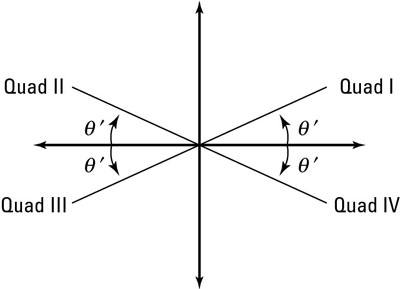
\includegraphics{reference}
\caption{Reference angles, sometimes call $\theta'$ (nothing to do with derivatives!)}
\end{center}
\end{figure}


\subsection{Trigonometric functions}
Also since ancient times, it has been exceedingly helpful to reference the ratios of
various components of an angle.  On a right triangle, these ratios are often memorized with
the helpful acronym S.O.H.C.A.H.T.O.A., short for sine = opposite/hypotenuse , cosine = 
adjacent/hypotenuse, tangent = opposite over adjacent.

\begin{figure}[h]
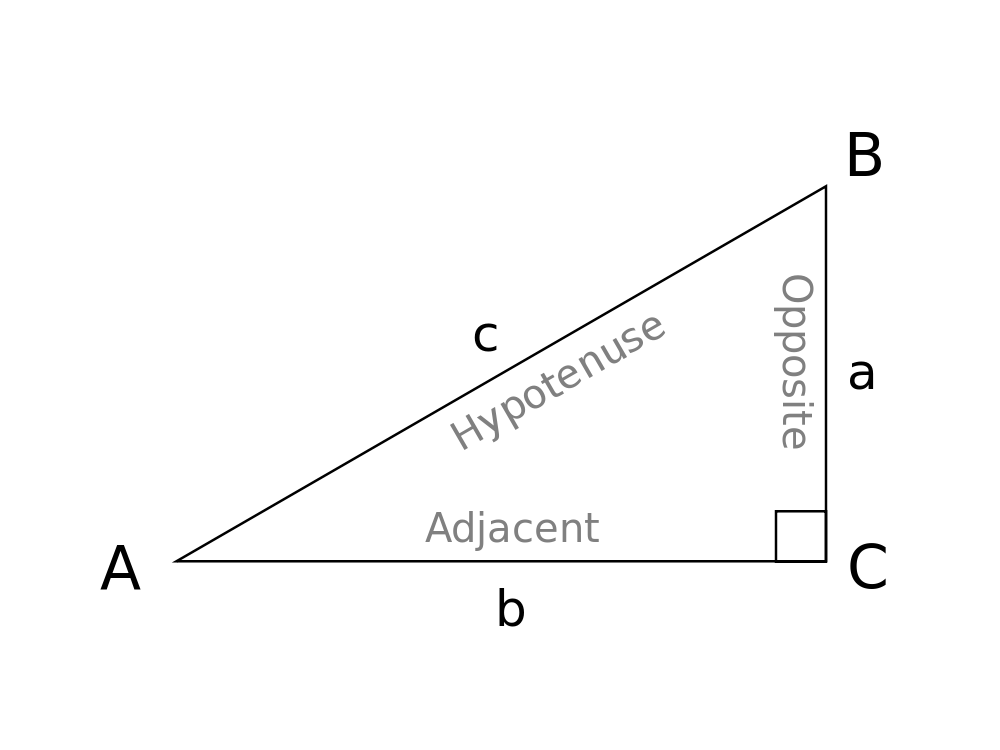
\includegraphics[scale=0.5]{TrigonometryTriangle.png}
\caption{The names of the sides of a right triangle}
\end{figure}

These definitions can be extended via reference angles to the other quadrants.  In 
such a context, the sine of an angle 
becomes the signed vertical displacement over the exact distance, cosine of an
angle becomes the signed horizontal displacement over the exact distance,
and tangent of the angle becomes its slope.

While no longer of much use or interest, there are names for the reciprocals of
the three main trigonometric functions.  The reciprocal of cosine is called
secant, the reciprocal of sine is called cosecant, and the reciprocal of tangent
is called cotangent.  Of these, only secant is commonly used (outside of math
classrooms!).


\newpage
\subsection{Exercises}
in Kuta



%									9 - 2
\newpage
\section{Reference Triangles}
\noindent\makebox[\textwidth]{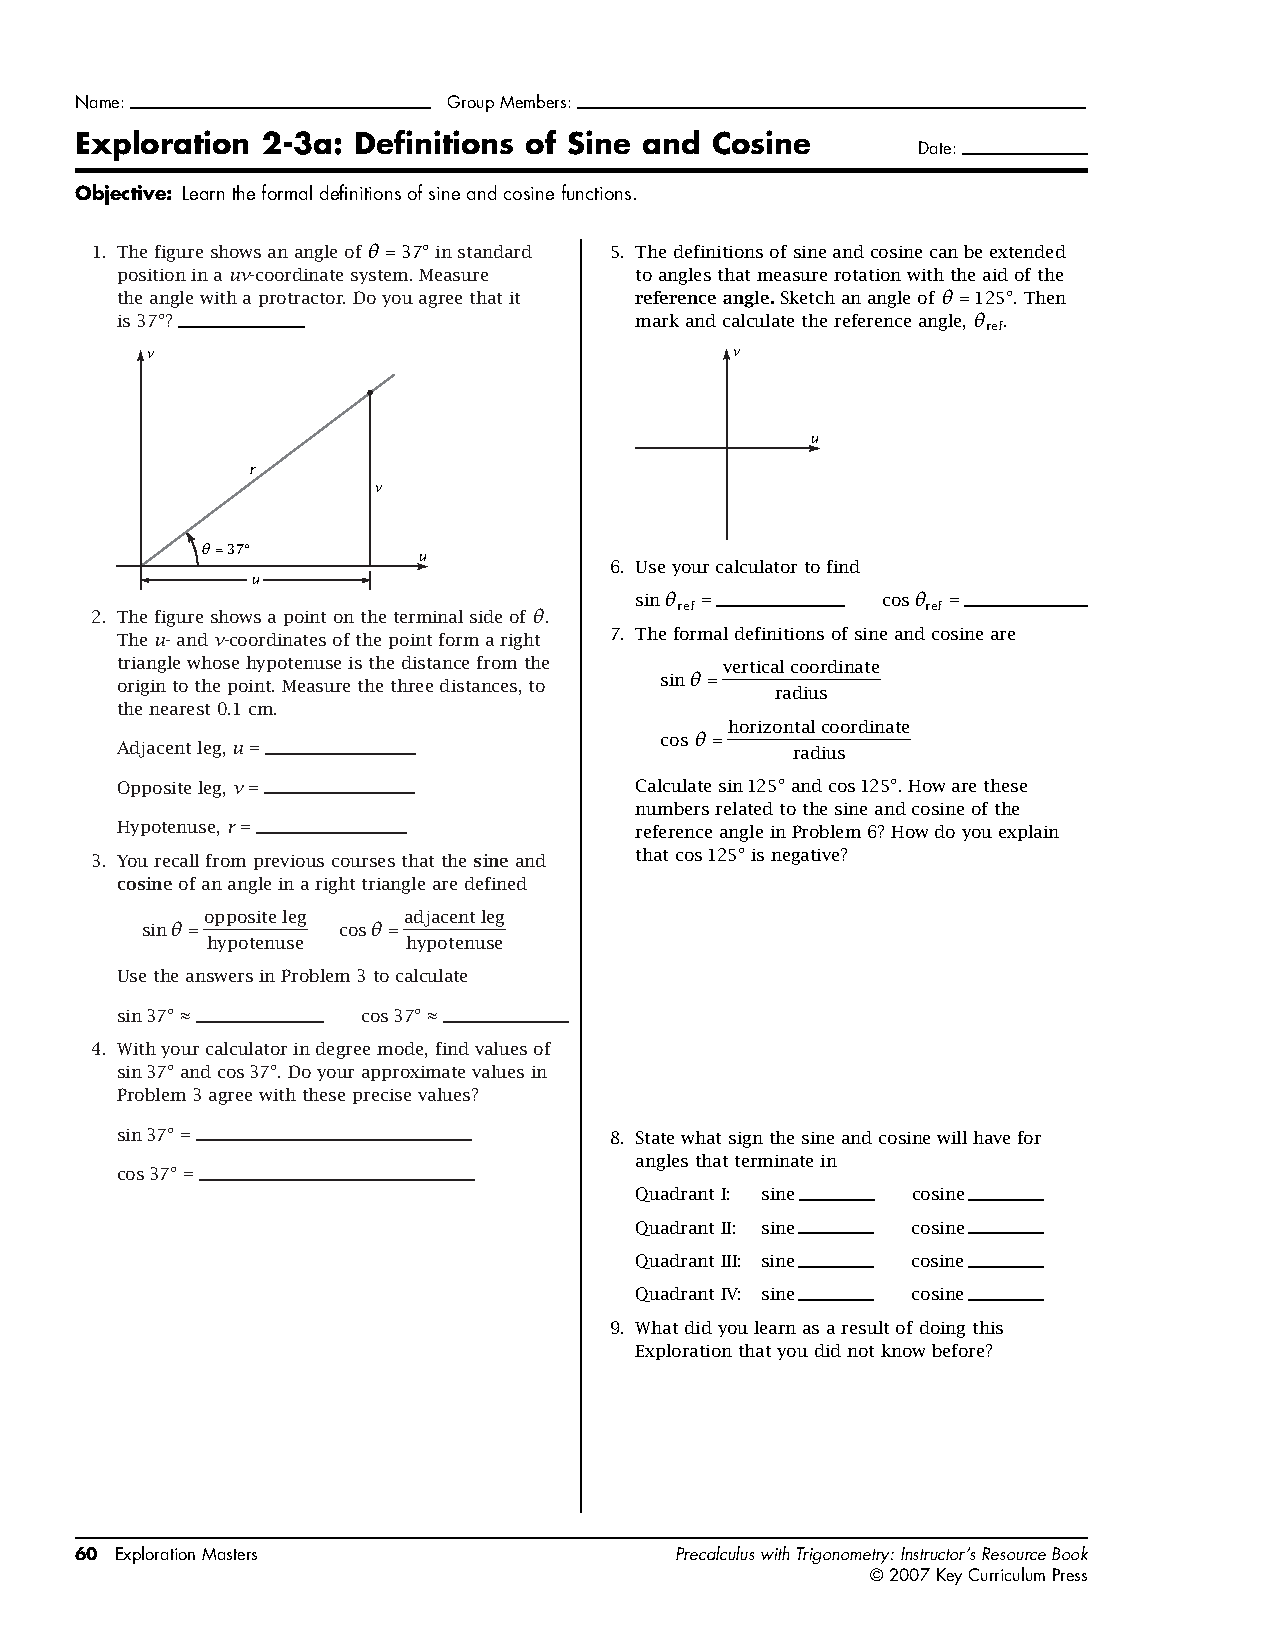
\includegraphics[width=\paperwidth]{ch09/0902p.pdf}}
\subsection{Special Triangles}
%!TEX root =  ../main.tex


\objective{Utilize standard angle values and circular symmetry}


There are not many angles we could draw for which we could precisely name
the displacement involved.  Two shapes we know every such thing about are the 
square and the equilateral triangle.  We might begin by drawing a square with
sides of length 1, and then drawing a diagonal.

\begin{figure}[h]
\begin{center}
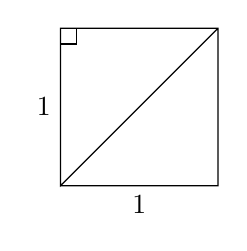
\begin{tikzpicture}[scale=2]
	\draw (0,0) -- (1,0) -- (1,1) -- (0,1) -- (0,0) -- (1,1);
	\draw (0,0.9) -- (.1,.9) -- (.1,1);
	\node at (0.5,0) [anchor=north] {1};
	\node at (0,0.5) [anchor=east] {1};
\end{tikzpicture}
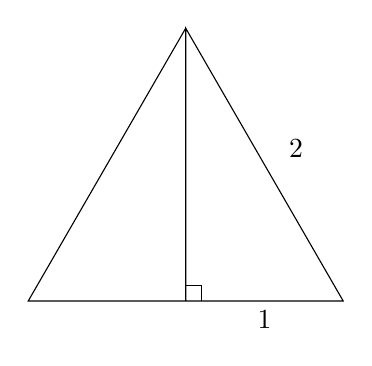
\begin{tikzpicture}[scale=2]
	\draw (0,0) -- (2,0) -- (1, 1.732050808) -- (1,0) -- (0,0) -- (1,1.732050808);
	\draw (1,.1) -- (1.1,.1) -- (1.1,0);
	\node at (1.5,0) [anchor=north] {1};
	\node at (1.7,.85) [anchor=south]{2};
\end{tikzpicture}
\caption{Special triangles are halves of thoroughly understood shapes.}
\end{center}
\end{figure}

According to the Pythagorean Theorem, what must the length of the 
hypotenuse be?  For either one of the triangles, what are the angles and
the ratios of the sides?

Next, consider an equilateral triangle with side of length 2.  If all the angles
are the same, what must they be?  Now we draw the perpendicular bisector,
which is also the altitude.  How long are the two half of the side we 
bifurcated?  What are the angles we split in two?  What would Pythagorus
tell you the length of the altitude is?

\begin{derivation}{Special Triangles}
The special triangles are derived from
squares and equilateral triangles.

A $45^\circ$-$45^\circ$-$90^\circ$ triangle has sides with ratios $1:1:\sqrt{2}$.

A $30^\circ$-$60^\circ$-$90^\circ$ triangle has sides with ratios $1:\sqrt{3}:2$.
\end{derivation}

Armed with such triangles, we can answer what sine, cosine, and tangent are
for $30^\circ$, $45^\circ$, and $60^\circ$, nine facts you should memorize.

\subsection{Reflection and Symmetry}
In the previous section of this chapter, we computed reference angles without
explaining why.  We will rectify that now.  Consider that there is a point $(x,y)$
somewhere in the first quadrant.  Draw a ray from the origin through this point,
and make it the terminal side of an angle.  Call that angle $\theta$.

\begin{figure}[h]
\begin{centering}
\begin{tikzpicture}[scale=0.5]
	\draw[<->, thick] (-4,0) -- (4,0);
	\draw[<->, thick] (0,-4) -- (0,4);
	\draw[fill] (55:3) circle (0.1) node[anchor=south] {$(x,y)$};
	\draw (3,0) arc(0:55:3);
	\node at (1,0.7) {$\theta$};
	\draw (0,0) -- (55:3);
\end{tikzpicture}
\caption{Turning angle $\theta$ results in going to coordinates $(x,y)$.}
\end{centering}
\end{figure}

What will be at the reference angle in the fourth quadrant?  If we turn
down from $0^\circ$ to $360^\circ-\theta$, we will be taken to $(x,-y)$.
In the second quadrant, the reference angle is $1800^\circ-\theta$, which
ends in the coordinates $(-x,y)$.  Finally, the third quadrant reference
angle of $180^\circ+\theta$ points to $(-x,-y)$.

Through the use of symmetry and reference angle, every fact we
learn in the first quadrant instantly reveals three other facts around
the grid.  Fill knowledge of the first quadrant entails full knowledge
of the entire Cartesian plane.

\begin{figure}[h]
\begin{centering}
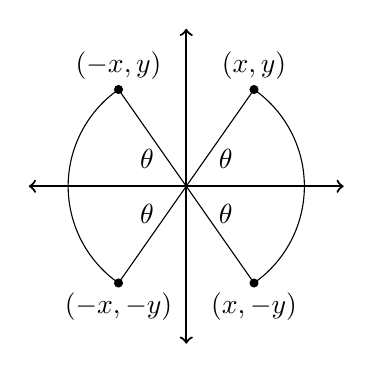
\begin{tikzpicture}[scale=0.5]
	\draw[<->, thick] (-4,0) -- (4,0);
	\draw[<->, thick] (0,-4) -- (0,4);
	
	\draw[fill] (55:3) circle (0.1) node[anchor=south] {$(x,y)$};
	\draw (3,0) arc(0:55:3);
	\node at (1,0.7) {$\theta$};
	\draw (0,0) -- (55:3);

	\draw[fill] (125:3) circle (0.1) node[anchor=south] {$(-x,y)$};
	\draw (0,0) ++ (125:3) arc(125:180:3);
	\node at (-1,0.7) {$\theta$};
	\draw (0,0) -- (125:3);

	\draw[fill] (235:3) circle (0.1) node[anchor=north] {$(-x,-y)$};
	\draw (0,0) ++ (180:3) arc(180:235:3);
	\node at (-1,-0.7) {$\theta$};
	\draw (0,0) -- (235:3);

	\draw[fill] (-55:3) circle (0.1) node[anchor=north] {$(x,-y)$};
	\draw (3,0) arc(0:-55:3);
	\node at (1,-0.7) {$\theta$};
	\draw (0,0) -- (-55:3);
\end{tikzpicture}
\caption{Reference angles are examples of horizontal and/or vertical symmetry. }
\end{centering}
\end{figure}


\subsection{$x$ and $y$ and slope}
Even the infinite number of points in the first quadrant can be scaled
down somewhat.  Let us consider only the points 1 unit away from
the origin.  Such points make a circle, called the Unit Circle.
If you think of sine as opposite over hypotenuse, and the hypotenuse is 
always 1, then on the unit circle, sine equals the opposite leg
of the reference triangle.  On the unit circle, this is always the $y$
value.  Sine \emph{is} $y$.

Again, if cosine is adjacent over hypotenuse and the hypotenuse is 
always one, then on the unit circle, cosine equals the adjacent leg
of the reference triangle.  On the unit circle, this always the $x$
value.  Cosine \emph{is} $x$.

Lastly, if tangent is opposite over adjacent, then on the unit circle
that is $y$ over $x$, rise over run, a.k.a. slope.  Tangent \emph{is}
slope.  And for any radius greater or less than 1, we need only 
multiply by that radius.  

When we overlay this way of thinking about trigonometric functions
(cosine is $x$, sine is $y$, tangent is slope) onto the grid, we can see
that all the first quadrant information we might gather can be
applied to any other quadrant with only sign changes.  Sine (as $y$)
will be positive in the first and second quadrant, and negative in
the third and fourth.  Cosine (as $x$) will be positive in the first
and fourth quadrants, and negative in the second and third.
Tangent (as $m$) will be positive in the first and third, and negative
in the second and fourth.


~\vfill
\newpage
\subsection{Exercises}
in Kuta
~\vfill

%									9 - 3
%\newpage
\section{Radians}
\noindent\makebox[\textwidth]{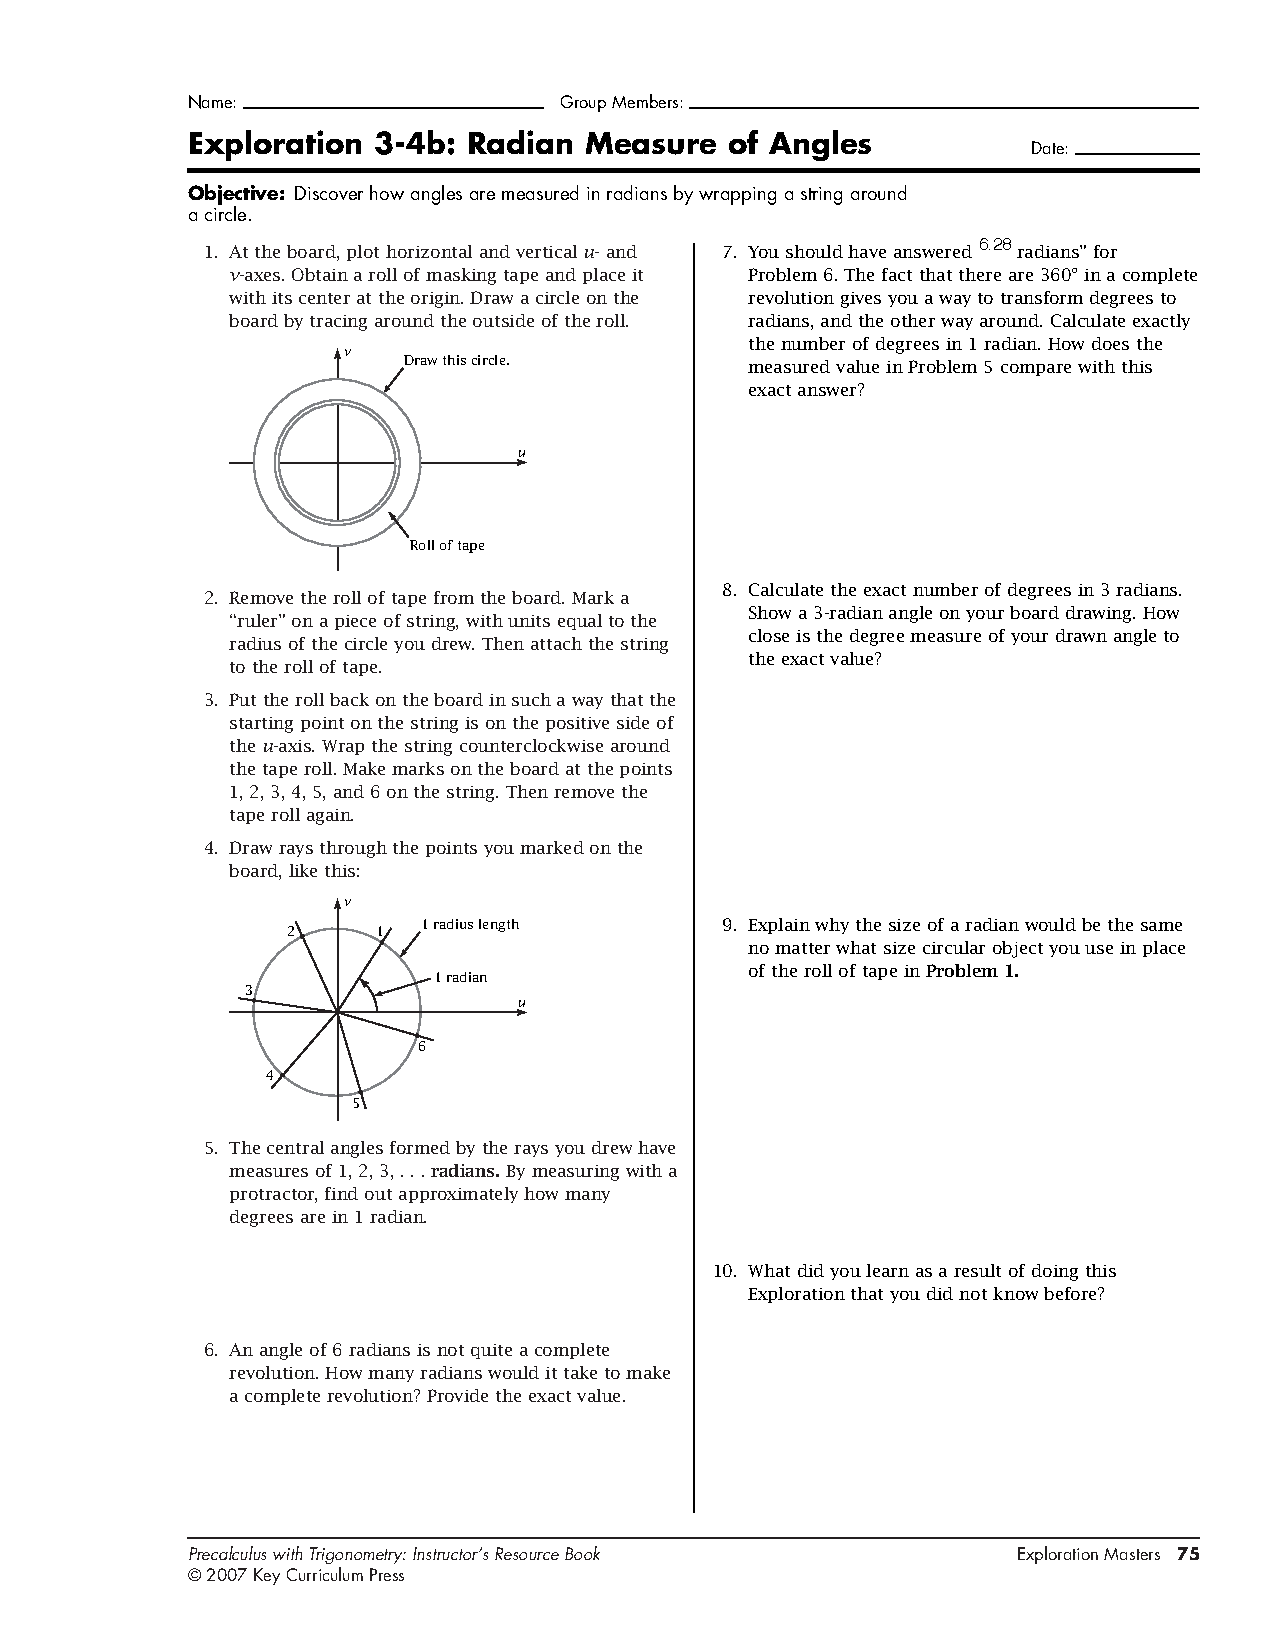
\includegraphics[width=\paperwidth]{ch09/0903p.pdf}}
\newpage
%!TEX root = ../main.tex

\subsection{Tau}
360 is nice enough number.  It divides evenly by 2, 3, 4, 5, 6, 8, 9, 10, 12, 15, 18, 20, 24, 30,
36, 40, 45, 60, 72, 90, and 180.  No other number under 1000 even comes close.  But it
is still arbitrary.  Why are there 60 seconds in a minute, 60 minutes in an hour, 360 degrees
in a full rotation?  Because Babylonian mathematicians wanted numbers that were easier
division!

A far more natural system exists and is indeed the only one used in calculus and higher
mathematics today.  Rather than assigning an arbitrary number to the complete
circle, we ask instead, what fraction of a full rotation have you turned?  One full rotation
will correspond with the entire circumference of the circle.  And again, this will be
done on the Unit Circle, so that an angle's measure is defined as the arc length
divided by the radius.  Because this is length divided by length, angles in this system
(called radians) have no units.  Turning all the way around one time is the same as
laying the radius of any circle out in a curved piece $6.28\dots$ times.  Rather than
write this irrational number to some arbitrary number of decimals, we use the symbol
$\tau$, called TAU.

There are no calculators with the number $\tau$ on them (yet), so we must use 
the fact that $\tau=2\pi$.

\subsection{Unit Circle}
This all culminates in the single figure that most embodies trigonometry: the completed
Unit Circle.  Because your education up to this point has utilized degrees, they are included
but you should concentrate on using radians, as they will be the main system used
from now on.  

\begin{figure}
\begin{center}
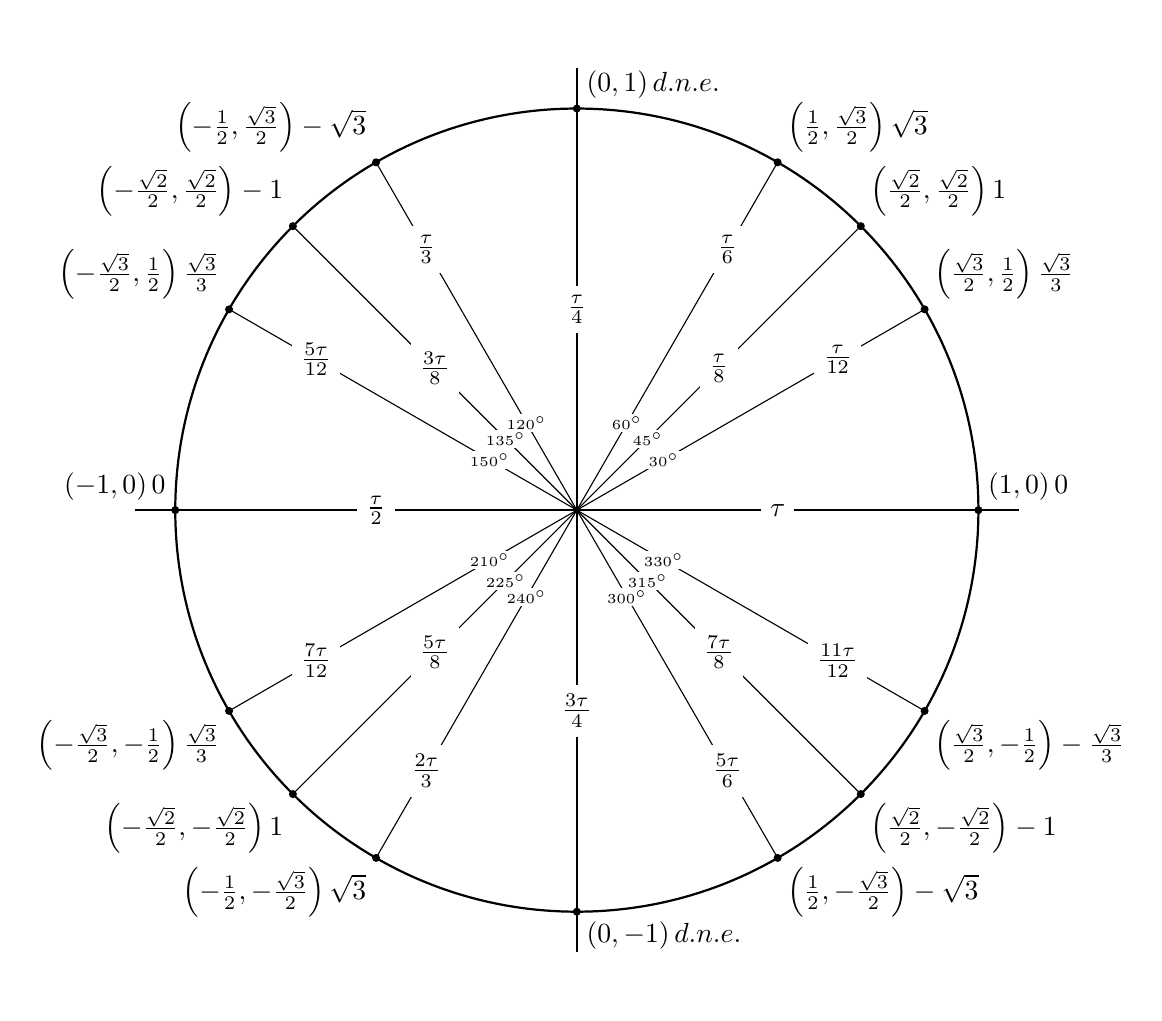
\begin{tikzpicture} [scale=1.7,
% Toggle commenting on the next four lines for the completed unit circle:
angle/.style={draw,text=white,fill=white,minimum height=1cm, minimum width=1cm},
point/.style={white},
angle/.style={fill=white},
point/.style={},
]
    \draw [white] (-3.6,-3.6) rectangle (3.6,3.6);
    \draw [thick,fill=white] (0,0) circle (3cm);
    \draw [thick, ] (-3.3,0) -- (3.3,0);
    \draw [thick, ] (0,-3.3) -- (0,3.3);
    \draw (0,0) --  node [angle] {$\frac{\tau}{4}$} (90:3)
                node[point, above right] {$ \left(0,1\right)  d.n.e.$};
    \draw (0,0) --  node [angle] {$\frac{\tau}{2}$} (180:3)
                node[point, above left] {$ \left(-1,0\right) 0$};
    \draw (0,0) --  node [angle] {$\frac{3\tau}{4}$} (270:3)
                node[point, below right] {$ \left(0,-1\right) d.n.e.$};
    \draw (0,0) --  node [angle] {$\tau$} (0:3)
                node[point, above right] {$ \left(1,0\right) 0$};
    \draw (0,0) --  node [angle] {$\frac{\tau}{8}$} (45:3)
                node [point, above right] {$ \left( \frac{\sqrt2}{2} , \frac{\sqrt2}{2}  \right) 1$};
    \draw (0,0) --  node [angle] {$\frac{3\tau}{8}$} (135:3)
                node [point, above left] {$ \left( -\frac{\sqrt2}{2} , \frac{\sqrt2}{2}  \right ) -1$};
    \draw (0,0) --  node [angle] {$\frac{5\tau}{8}$} (225:3)
                node [point, below left] {$ \left( -\frac{\sqrt2}{2} , -\frac{\sqrt2}{2}  \right) 1$};
    \draw (0,0) --  node [angle] {$\frac{7\tau}{8}$} (315:3)
                node [point, below right] {$ \left( \frac{\sqrt2}{2} , -\frac{\sqrt2}{2}  \right) -1$};
    \draw (0,0) --  node [near end, angle] {$\frac{\tau}{12}$} (30:3)
                node [point, above right] {$ \left( \frac{\sqrt3}{2} , \frac{1}{2}  \right) \frac{\sqrt{3}}{3}$};
    \draw (0,0) --  node [near end, angle] {$\frac{\tau}{6}$} (60:3)
                node [point, above right] {$ \left( \frac{1}{2} , \frac{\sqrt3}{2}  \right) \sqrt{3} $};
    \draw (0,0) --  node [near end, angle] {$\frac{\tau}{3}$} (120:3)
                node [point, above left] {$ \left( -\frac{1}{2} , \frac{\sqrt3}{2}  \right) -\sqrt{3} $};
    \draw (0,0) --  node [near end, angle] {$\frac{5\tau}{12}$} (150:3)
                node [point, above left] {$ \left(- \frac{\sqrt3}{2} , \frac{1}{2}  \right) \frac{\sqrt{3}}{3} $};
    \draw (0,0) --  node [near end, angle] {$\frac{7\tau}{12}$} (210:3)
                node [point, below left] {$ \left(- \frac{\sqrt3}{2} , -\frac{1}{2}  \right) \frac{\sqrt{3}}{3}$};
    \draw (0,0) --  node [near end, angle] {$\frac{2\tau}{3}$} (240:3)
                node [point, below left] {$ \left( -\frac{1}{2} , -\frac{\sqrt3}{2}  \right) \sqrt{3}$};
    \draw (0,0) --  node [near end, angle] {$\frac{5\tau}{6}$} (300:3)
                node [point, below right] {$ \left( \frac{1}{2} , -\frac{\sqrt3}{2}  \right) -\sqrt{3}$};
    \draw (0,0) --  node [near end, angle] {$\frac{11\tau}{12}$} (330:3)
                node [point, below right] {$ \left( \frac{\sqrt3}{2} , -\frac{1}{2}  \right) -\frac{\sqrt{3}}{3}$};
 
    \foreach \n in {1,2,3,4}
        \foreach \t in {0,30,45,60}
            \fill (\n*90+\t:3) circle (0.03cm);
    \foreach \t in {30,45,60, 120,135,150, 210,225,240, 300,315,330}
        \node [font=\tiny, fill=white,inner sep=1pt] at (\t:.75) {$ \t^\circ $};
\end{tikzpicture}
\caption{The full unit circle, with $x$, $y$, and $m$, radians and degrees, for your careful study.}
\end{center}
\end{figure}


It may be helpful to think of conversion to and from radians as dimension analysis,
as in the sciences.  A full circle is 1 $\tau$, which is the same as $360^\circ$, so these
numbers can be put in a fraction equalling one.  Multiplying by one does not change 
anything.

\begin{example}{Conversion}
\exProblem
Convert $215^\circ$ into radians and $\frac{5\tau}{6}$ into degrees

\exSolution
$$
215^\circ \cdot \frac{\tau}{360^\circ} = \frac{215\tau}{360} = \frac{43\tau}{72}
$$
and
$$
\frac{5\tau}{6} \cdot \frac{360^\circ}{\tau} = \frac{1800^\circ}{6} = 300^\circ
$$
\end{example}

\subsection{Derivative}
We have already said that sine is y, cosine is x, and tangent is m, but m (slope)
is y over x, so tangent is sine over cosine.  Recall that the reciprocals of the
standard trigonometric functions have names, specifically that 1 over sine
is cosecant, 1 over cosine is secant, and 1 over tangent is cotangent.  You are asked
to find the derivatives of each in the exercises.

While it is not the formal proof for the derivative of sine we will present in chapter
\ref{ch:identities}, we can now build a geometric proof.  Sine is the signed vertical
displacement of a point on the unit circle, after we have traversed $\theta$ units of
arc.  For every tiny nudge $d\theta$, there is a similar triangle created that
highlights the additional change brought about to the height, or $\sin\theta$.  The 
figure below shows how on the smaller triangle, the ratio of the adjacent side
to the hypotenuse -- cosine -- is tiny change in the height.  All these values
become more accurate the smaller the triangle becomes.

\begin{figure}[h]
\begin{centering}
\begin{tikzpicture}[line cap=round,line join=round,x=2cm,y=2cm,
     spy using outlines={rectangle,lens={scale=12}, size=8cm, connect spies}]
	\coordinate (A) at (30:2);
	\coordinate (B) at (1.73205,0);
	\coordinate (C) at (1.672,1.1000);
	\coordinate (D) at (1.672,1.0000);
	\draw[->] (-0.5,0) -- (2.2,0) node[anchor=west] {$x$};
	\draw[->] (0,-0.3) -- (0,2.1) node[anchor=west] {$y$};
	\draw(0,0) ++ (-10:2) arc (-10:100:2.01);
	\draw(0,0) -- (A) -- (B);
	\draw(C) -- (D) -- (A);
	\draw[ultra thin](0,0) ++ (0:2.2) arc (0:30:2.2) ;

	\node at (2.3,0.5) {$\theta$};
	\spy [blue] on (1.7,1.05)
             in node [left] at (6.5,1);
	\draw[decorate, decoration={brace},xshift=0.5cm,yshift=0.4cm] (4.2,1.6) -- (4.9,0.4) node[midway,xshift=0.5cm,yshift=0.2cm] {$d\theta$};
	\draw (4.2,1.6) ++ (-90:.5) arc (-90:-60:0.5) node[midway,yshift=-0.2cm] {$\theta$};
	\draw[decorate, decoration={brace},xshift=-0.5cm] (4.2,0.4) -- (4.2,1.6) node[midway,xshift=-0.6cm] {$\cos\theta$};
\end{tikzpicture}
\caption{Zoom in on $\theta$ plus a tiny $d\theta$'s effect on $\sin\theta$.}
\end{centering}
\end{figure}




\newpage
\subsection{Exercises}
in Kuta in two parts
~\vfill


%									9 - 4
%\newpage
\invisiblesection{Graphs}
\subsection{Problems}
\noindent\makebox[\textwidth]{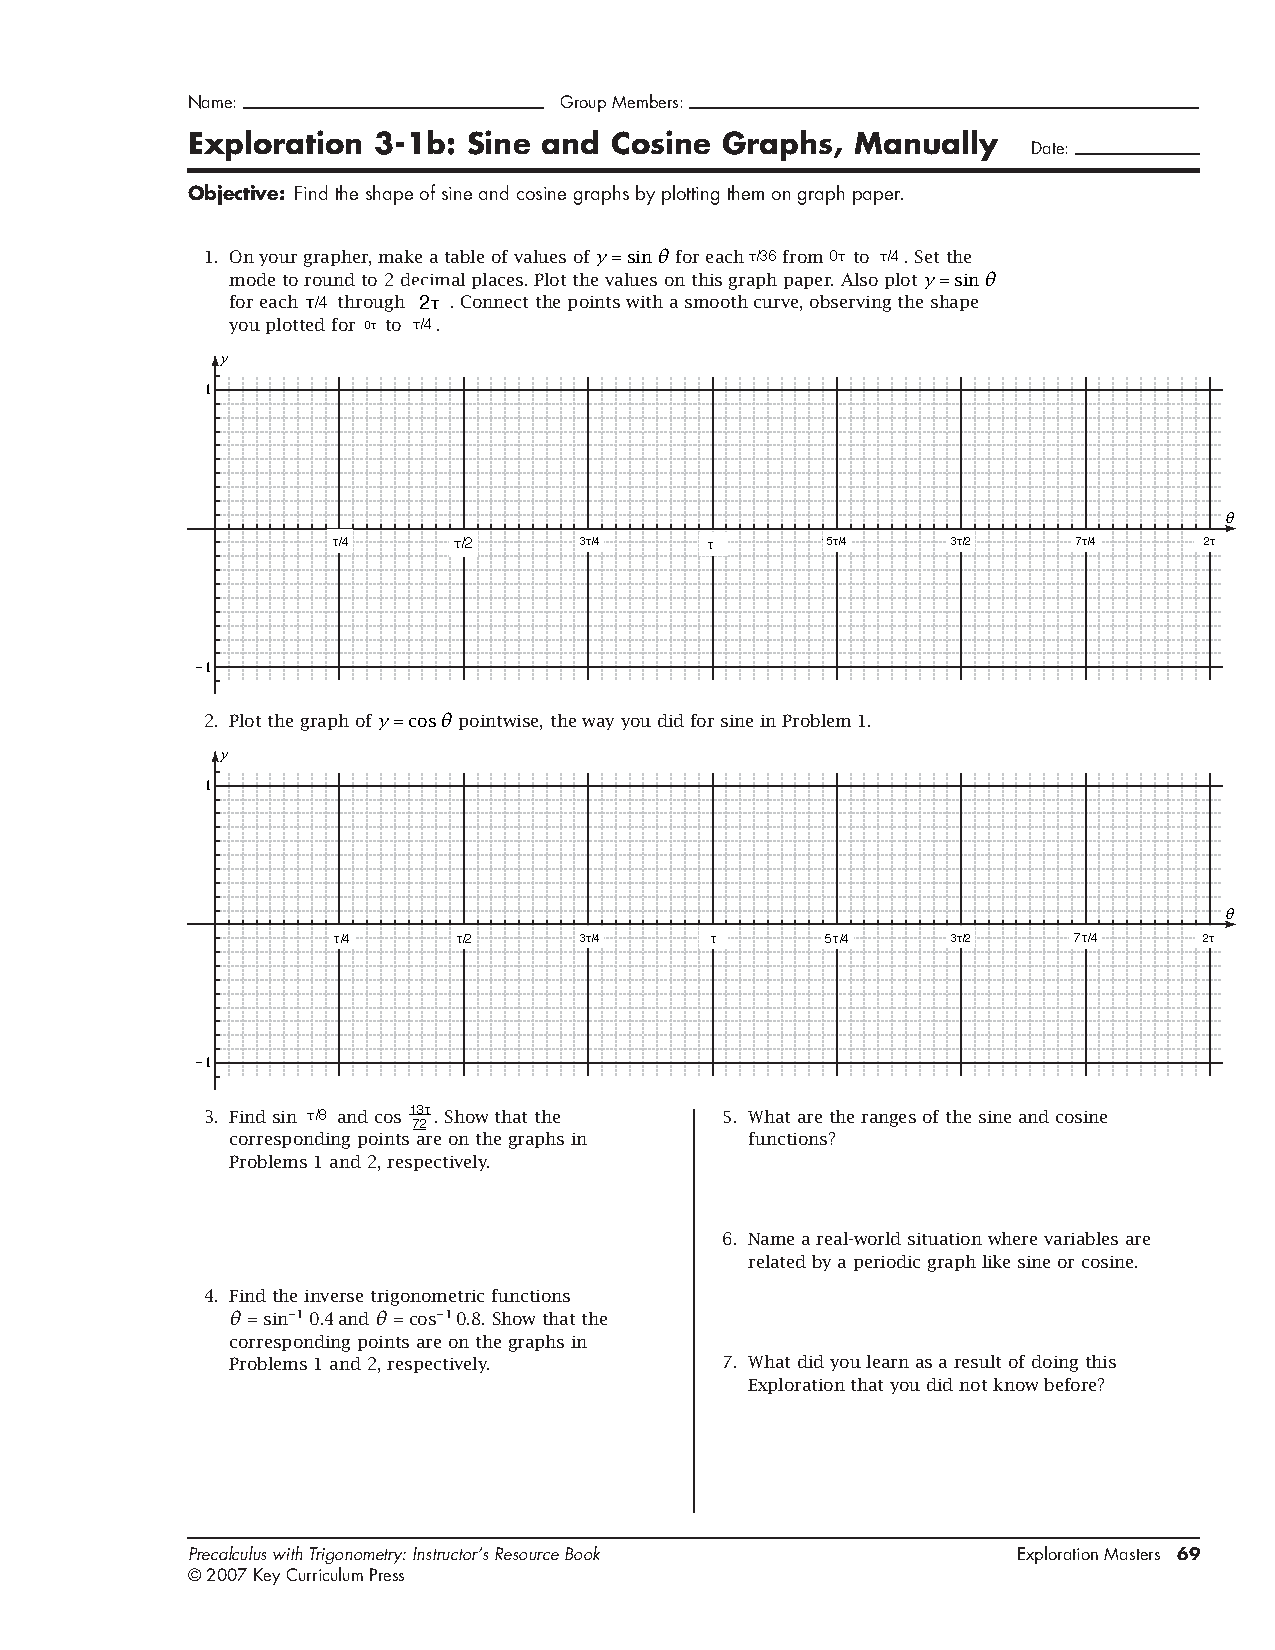
\includegraphics[width=\paperwidth]{ch09/0904p.pdf}}
%!TEX root =  ../main.tex

\subsection{$xy\theta$}

\objective{Produce and derive trigonometric function graphs}


On a piece of paper or on the screen of an electronic device, we typically graph only two
variables.  3D graphs are usually ``faked'', as in orthographic projections or the like.  The 
Unit Circle is actually three things graphed at once, and so somewhat obscures each:
the height (sine), the width (cosine), and the angle turned ($\theta$).  We will tease apart
various attributes of the Unit Circle and their relationships to $\theta$, in order to understand
each more clearly.

\subsubsection{$y\theta$}
\marginfig[-0in]{\chapdir/pics/TIsinx}{$y=\sin(x)$ on the TI-8*}
If we graph the height we have ascended to as the dependent variable, and the angle we
have turned as the independent variable, this corresponds to $y=\sin(x)$.  This is a good
beginning, because we are graphing the $y$ of the Unit Circle as a our $y$, but we have
changed the $x$ to $\theta$.  Enter this equation in your TI-8* and hit ZOOM-TRIG, begin
sure to be in radians mode.

The graph has not been shifted up or down at all, so its midline or \textbf{axis} is the line
$y=0$.  The graph oscillates as much as one up or one down from that axis, so 1
is the \textbf{amplitude}.  We know that the pattern of the Unit Circle (relative to
the angle turned) takes $360^\circ$ or $\tau$ radians to repeat, so that should
be the \textbf{period}.  What has the calculator done to make us get back to the
same point on the way in four tick marks?  Press WINDOW, and you will see that
the Xscl is $1.57\dots$, a.k.a. $\frac{\tau}{4}$.

Notice how the graph spends a great deal of time near the origin looking like $y=x$.
In other words, its derivative at 0 is 1.  Practice moving your writing hand in a smooth
wave, tracing the unit circle at a consistent pace, but focusing your attention on your
height above and below the $x$-axis.  This should feel that same as tracing $y=\sin(x)$.
Because this graph is so ubiquitous in nature, anything like it is described with the
adjective \textbf{sinusoidal}, and anything which moves as it does is said to be in 
\textbf{simple harmonic motion}.

\subsubsection{$x\theta$}
A cosine graph is very, very similar.  Tracing the Unit Circle while focusing on your
$x$ position is nearly identical, except the cycle begins on 1.  Change you TI-8* to
$y=\cos(x)$ but change nothing else.  Now you are graphing $x$ from the Unit Circle
on $y$, and $\theta$ from the Unit Circle on $x$.

\begin{example}{Watermill}
\exProblem
A mill is powered by a water-wheel in a river, which is 12 feet in diameter.  You observe
that it takes 20 seconds to complete a rotation and only the bottom 1ft is in the water.
There is a flag or marker at the top of the wheel right now.
Create an equation to model the water-wheels behavior, graph it, and determine the
time the flag will go into the water, and how long it spends underwater each rotation.


\exSolution

We begin by reasoning from the Unit Circle to the water-wheel.  Unit Circle graphs have an
amplitude of 1 because the are waves on a circle of radius 1.  The water-wheel has
a radius of 6 ft, so that will be our amplitude.  Graphically, that would make our wave
six times taller than normal, so we need a vertical dilation of 6.  So far we have
$$
y=6\sin(x)
$$
\marginfig[-0in]{\chapdir/pics/6sinx}{$y=6\sin(x)$}
Which produces a graph as in Fig.~\ref{fig:6sinx}.  The water-wheel must have its axis
translated, if only the bottom 1ft is in the water.  With an amplitude of 6ft, our current
version is 5ft too low, so we can revise our equation to $y=6\sin(x)+5$.  We also note
that as a sine wave, our graph begins in the middle and is rising, whereas we need to
model an object beginning at the top.  Therefore, we switch our equation to a cosine 
function.

The normal period of a sinusoidal wave is $\tau$, but we need the period to be 20.
Horizontal dilation is accomplished by dividing --- not multiplying, as in vertical
dilation --- so we must ask what to divide $\tau$ by in order to get 20.  The answer is
$\frac{\tau}{20}$.  Our final equation is (including the form we must use in the TI-8*):
$$
y=6\cos\frac{\tau}{20}(x)+5 = 6\cos\frac{\pi}{10}(x)+5
$$

According to the zero function of the grapher, the height is zero at $x=8.135705$
and again at $x=11.864295$, meaning the flag will go under just after 8 seconds
from now, and be underwater for a little less than 4 seconds.

\marginfig[1in]{\chapdir/pics/waterwheelgraph}{The entire mill setup visualized}
\end{example}


\newpage
\subsection{Exercises}
in Kuta


%									9 - 5
\newpage
\invisiblesection{Inverse Trigonometric Functions}
\subsection{Problems}
\noindent\makebox[\textwidth]{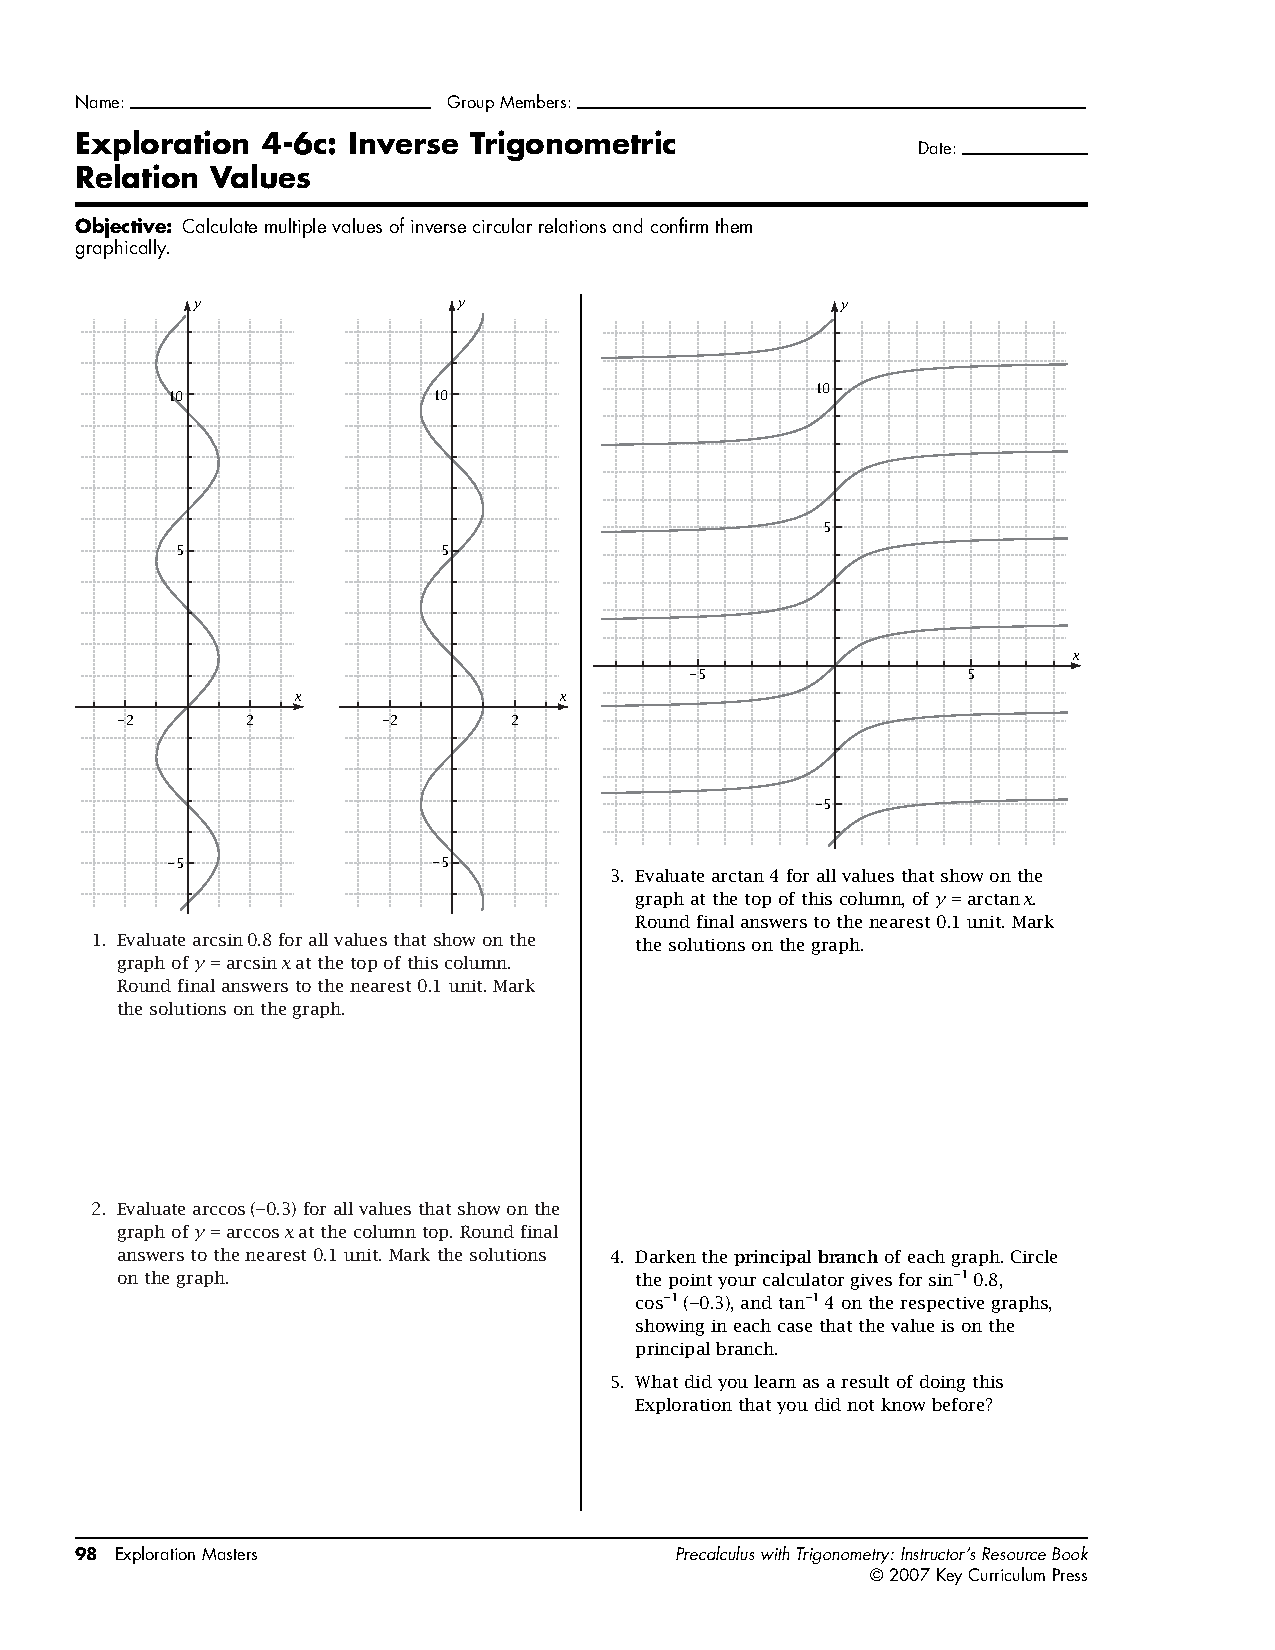
\includegraphics[width=\paperwidth]{ch09/0905p.pdf}}
%!TEX root =  ../main.tex

\objective{Use but also know the limitations of inverse trigonometric functions}


The standard trigonometric functions work by receiving angles as input, and outputting
the appropriate ration of side from the Unit Circle.  Often, we need have the ratio of sides
and wish to know the angle that must exist between them.  Thinking in terms of functions,
this is the inverse of the normal, asking for the input corresponding to a given output.
But as we saw last section, the trigonometric functions all have an infinite number of
repetitions of each output.  They are not invertible.

That is to say, they do not invert to functions across their entire domains.  We must limit
their possible input if their inverses are to be functions.  The criteria of deciding the
inverse domains are:
\begin{itemize}
\item All possible outputs must be represented
\item Be as continuous as possible
\item Be centered around the origin
\end{itemize}

insert 6 inverse relations and highlighted ranges

insert unit circle with relevant semi-circles

\subsection{Composing}
\subsubsection{Inverse inside Normal}
It is straight-forward to interpret $\sin(\sin^{-1}(\frac{1}{2}))$:  ``What is sine when
sine is one-half?''  Very easy: it is one-half!  What about $\sin(\cos^{-1}(\frac{1}{2}))$?
``What is sine, when cosine is one-half?''  We could fine the angle were cosine has that
value ($60^\circ$) and take the sine of that angle, but we could also recognize that
arccosine is giving us adjacent-over-hypotenuse, and sine is asking for opposite-over-hypotenuse,
and easy problem to solve with Pythagorus's help.  It is $\frac{\sqrt{3}}{2}$.

The second approach --- drawing a right triangle with two of the side-lengths known --- is
a much more power tool and extendable to more circumstances.  Consider 
$\cos(\sin^{-1}(x))$.  ``What is cosine when sine is $x$?''  Again, sine is giving us
adjacent over hypotenuse.  We can imagine a right-triangle with one angle, call it
$\theta$.  Sine of $\theta$ means the adjacent is $x$ and the hypotenuse is 1.
The Pythagorean Theorem will allow is to find the opposite: it must be $\sqrt{1-x^2}$.

\begin{figure}
\begin{centering}
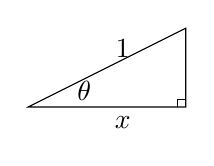
\begin{tikzpicture}
	\draw (0,0) -- (2,0) -- (2,1) -- cycle;
	\node (A) at (1.2,0) [anchor=north] {$x$};
	\node (B) at (1.2,.5) [anchor=south] {1};
	\node (C) at (.5,.2) [anchor=west] {$\theta$};
	\draw (1.9,0) -- (1.9,.1) -- (2.0,.1);
\end{tikzpicture}
\caption{A visualization of $\cos(\sin^{-1}(x))$.}
\end{centering}
\end{figure}

\subsubsection{Normal inside Inverse}
Perhaps you would be surprised at the answer if you put $\sin^{-1}(\sin(3))$ into your
TI-8*.  Would you expect it to answer 3?  How can we verbalize what this expression
is asking?  ``Extend an arc 2 units and record the resulting height above the $x$-axis.
What angle produces this height above the $x$-axis?''  We could interpret it visually
on the unit circle like this:

\begin{figure}[h]
\begin{centering}
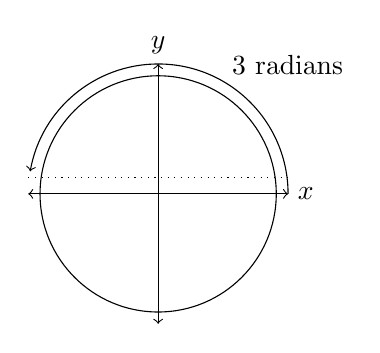
\begin{tikzpicture}[scale=1.5]
	\draw[<->] (-1.1,0) -- (1.1,0) node [anchor=west] {$x$};
	\draw[<->] (0,-1.1) -- (0,1.1) node[anchor=south] {$y$};
	\draw (0,0) circle (1);
	\draw[->] (0,0) ++ (0:1.1) arc (0:170:1.1) node[midway,xshift=1.5cm] {3 radians};
	\draw[dotted] (-1.1,0.14) -- (1.1,0.14);
\end{tikzpicture}
\caption{3 radians is a height arcsine can find in \texttt{QI}.}
\end{centering}
\end{figure}

Notice that the height above the $x$-axis -- the sine of the angle -- is achievable in
the first quadrant.  Arcsine --- because it is a function and can only return one
value per input --- must answer a positive input in the first quadrant.

\subsection{Derivatives}
How can we find the derivatives of inverse trigonometric functions?  The
definitions of inverses is very helpful: swapping $x$ and $y$.  Inverse sine is just
$x=\sin(y)$.  Using implicit differentiation, we get $dx=\cos(y)dy$.  Therefore,
$$
\frac{dy}{dx} = \frac{1}{\cos(y)} = \frac{1}{\cos(\sin^{-1}(x))}
$$

As we saw above, this can be simplified.  You will find all six inverse trigonometric 
functions derivatives in the exercises.

\newpage
\subsection{Exercises}
in kuta in two parts

%									9 - 6
\newpage
\section{Review}
\subsection{Chapter Review}
\subsection{Chapter Test}